% Created 2022-04-02 Sat 19:52
% Intended LaTeX compiler: pdflatex
\documentclass[11pt]{article}
\usepackage[utf8]{inputenc}
\usepackage[T1]{fontenc}
\usepackage{graphicx}
\usepackage{grffile}
\usepackage{longtable}
\usepackage{wrapfig}
\usepackage{rotating}
\usepackage[normalem]{ulem}
\usepackage{amsmath}
\usepackage{textcomp}
\usepackage{amssymb}
\usepackage{capt-of}
\usepackage{hyperref}
\usepackage{tabularx}
\usepackage{minted}
\author{Adam Salwowski}
\date{\today}
\title{Statyczna strona portfolio wraz z poradnikami programistycznymi dla początkujących}
\hypersetup{
 pdfauthor={Adam Salwowski},
 pdftitle={Statyczna strona portfolio wraz z poradnikami programistycznymi dla początkujących},
 pdfkeywords={},
 pdfsubject={},
 pdfcreator={Emacs 27.1 (Org mode 9.3)}, 
 pdflang={Polish}}
\begin{document}

\maketitle
\tableofcontents

\section{Wstęp}
\label{sec:org058dcf7}
Strona portfolio prezentująca projekty programisty. Centrum informacji dla początkujących programistów w postaci poradników i treściwych objaśnień.
\subsection{Cel projektu}
\label{sec:org323519e}
\begin{itemize}
\item Dla pracodawcy
\begin{itemize}
\item pokazanie z jakimi typami programista miał do czynienia
\item pokazanie sposobu rozwiązywania problemów
\item pokazanie jak wygląda kod (czy jest schludny i czytelny, lub może chaotyczny)
\item pokazanie czy dobrze zna technologie
\item pokazanie czy zna najnowsze rozwiązania w programowaniu
\end{itemize}
\item Dla programisty
\begin{itemize}
\item pozwala uporządkować doświadczenie i przedstawić je lepiej niż w CV
\item pokazuje realne doświadczenie i wiedzę
\item pokazuje czego programista jeszcze nie robił i w jakim kierunku mógłby się jeszcze rozwinąć
\end{itemize}
\item Dla początkującego
\begin{itemize}
\item miejsce w którym może się zapoznać w dość szybkim czasie z wieloma technologiami
\end{itemize}
\end{itemize}
\subsection{Dla kogo ta aplikacja jest przeznaczona}
\label{sec:org3682795}
\begin{itemize}
\item firmy zatrudniające programisów
\item początkujący programiści
\end{itemize}
\subsection{Użyte technologie użyte podczas produkcji strony}
\label{sec:org8f9f1c5}
\begin{itemize}
\item apache / nginx
\item html
\item css
\item org-mode
\item VPS (Virtual Private Server)
\item deployment strony
\item obraz png (zdjęcie)
\end{itemize}
\subsection{Użyte technologie podczas produkcji dokumentacji}
\label{sec:org7cb9d0b}
\begin{itemize}
\item latex
\item org-mode
\end{itemize}
\subsection{Użyte technologie w celu dydaktycznym}
\label{sec:org465b9c6}
\begin{itemize}
\item instalacja niezbędnych pakietów
\item komendy unixowe:
\begin{itemize}
\item wget?
\item curl?
\item imagemagick?
\item ffmpeg?
\end{itemize}
\item konfiguracja środowiska programistycznego (edytor tekstowy Emacs)
\begin{itemize}
\item instalacja pakietów
\item przykładowe funkcje oraz ich działanie
\item obsługa magit?
\end{itemize}
\item python
\begin{itemize}
\item moduły:
\begin{enumerate}
\item argparse
\item pathlib
\item os
\item beautifulsoup4
\item requests
\end{enumerate}
\end{itemize}
\item html
\item css
\item java
\item c
\item c++
\item emacs lisp
\item latex
\item markdown
\item org-mode
\item regex
\item git
\end{itemize}
\section{Specyfikacja wymagań}
\label{sec:org9f3d099}
\subsection{Wymagania funkcjonalne systemu}
\label{sec:org814aa83}
\begin{verbatim}
w postaci zadań szczegółowych?? za długa linijka była
\end{verbatim}

\begin{description}
\item[{zarządzaj stroną}] pozwala na dokowynania operacji \textbf{CRUD} na stronie programisty
\item[{opłac hosting}] odpowiada za opłacenie serwisowi hostingu strony
\item[{wyświetl stronę}] odpowiada za wyświetlenie strony w przeglądarkce użytkownikom systemu
\end{description}
dlaczego z jakiej strony, administator
\subsection{Słownik pojęć systemowych}
\label{sec:org590a595}
\begin{description}
\item[{strona}] cała strona z treścią dla \emph{początkujących} oraz \emph{pracodawców}
\item[{poradniki}] część strony wyznaczona dla \emph{początkującego}, zawierająca tutoriale
\item[{portfolio}] część strony wyznaczona dla \emph{pracodawcy}, zawierająca treści interesujące \emph{interviewerów} zatrudniających do firm
\end{description}
\subsection{Specyfikacja grupy użytkowników}
\label{sec:orge0ef0b4}
\begin{center}
\begin{tabular}{llll}
Atrybut & Programista & Początkujący & Pracodawca\\
\hline
Wiek & brak & brak & brak\\
Umiejętności obsługi komputera & zaawansowane & średnie & zaawansowane\\
Wykształcenie & wyższe & podstawowe & wyższe\\
Znajomość tematyki SI & podstawowa & podstawowa & podstawowa\\
\end{tabular}
\end{center}
\subsection{Aktorzy}
\label{sec:org091554e}
\begin{description}
\item[{programista (ja)}] osoba odpowiedzialna za stworzenie strony
\item[{pracodawca}] lub także \emph{interviewer}, osoba odpowiedzialna za zatrudnianie do firmy, sprawdzająca korepetycje
\item[{początkujący}] osoba zaczynająca karierę w IT, ucząca się podstaw programowania na stronie \emph{programisty}
\item[{serwis hostingowy}] usługa, dzięki której strona \emph{programisty} będzie dostępna dla każdego w sieci
\item[{system płatności}] dzięku której, \emph{programista} ureguluje zapłatę z \emph{serwisem hostingowym} za usługę
\end{description}
\subsection{Diagram przypadków użycia}
\label{sec:org9f84e64}
\begin{figure}[htbp]
\centering
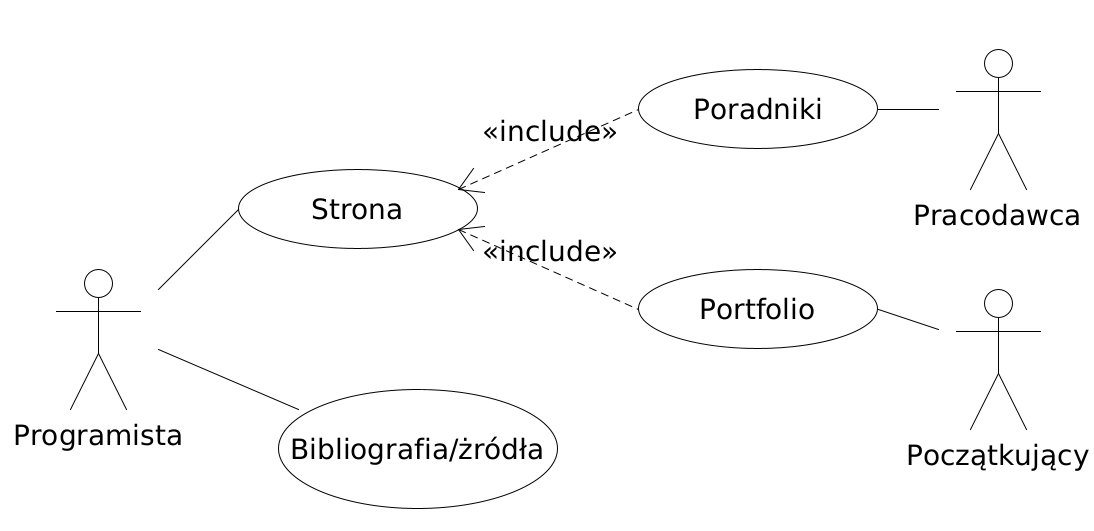
\includegraphics[width=.9\linewidth]{./images/diagram_przypadkow_uzycia.png}
\caption{Diagram przypadków użycia}
\end{figure}
\subsection{Diagram encji}
\label{sec:orge6cdeab}
qwe
\subsection{Diagram klas}
\label{sec:org7884d62}
qwe
\subsubsection{Atrybuty klas}
\label{sec:orgcddf231}
\begin{description}
\item[{Programista}] imie, nazwisko, e-mail, repozytoria, źródła
\item[{Początkujący}] imie, nazwisko, e-mail
\item[{Pracodawca/Interviewer}] imie, nazwisko, e-mail
\item[{Strona}] link, treść, technologie
\end{description}

\section{Użyte technologie}
\label{sec:orge0ecf99}
\subsection{opis używanych języków i technologii oprogramowania (html,css)}
\label{sec:orgf553df0}
\section{Interfejs użytkownika}
\label{sec:orga049521}
\subsection{Graficzna instrukcja użytkowania aplikacji}
\label{sec:org19ff35c}
\section{Podsumowanie efektu pracy}
\label{sec:orgcc13221}
\subsection{Jak można jeszcze rozwinąc aplikację w przyszłości}
\label{sec:orgda43569}
\subsection{Co się udało zrobić, a czego nie}
\label{sec:org4487dd1}
\section{Bibliografia}
\label{sec:org66283bb}
\subsection{Wykorzystane źródła}
\label{sec:org81b4f4a}
\subsubsection{Kanały youtube?}
\label{sec:orgcf6aaab}
\begin{itemize}
\item \url{https://youtube.com/channel/DistroTube}
\end{itemize}
\subsubsection{Strony internetowe}
\label{sec:org3ad41f8}
\begin{enumerate}
\item Strony portfolio
\label{sec:org8f2bfc4}
\begin{itemize}
\item \url{https://lukesmith.xyz}
\end{itemize}
\item Strony dydaktyczne
\label{sec:orgec41b09}
\begin{itemize}
\item \url{https://landchad.net}
\item \url{https://xahlee.info}
\end{itemize}
\end{enumerate}
\subsubsection{Książki}
\label{sec:orgc59a317}
\begin{itemize}
\item jakaś książka o emacs?
\item jakaś książka o
\end{itemize}
\subsubsection{Prezentacje?}
\label{sec:orgaaaf54b}
\subsection{nie tylko strony internetowy, mają być książki, prezentacje}
\label{sec:orgd2bc2da}
\section{Podsumowanie}
\label{sec:orgad7391f}
\end{document}